\section{Modelos projetados}
\subsection{Plantas}
Os robôs 1 e 2, possuem comportamentos similares, onde as rotinas de posicionamentos espaciais são projetadas em forma de funções, onde são acionadas através de sinais vindo do CLP (Controlador Lógico Programável).
Os movimentos do robô 1 consistem em:

\begin{enumerate}
  \item Pegar peça na mesa centralizadora, que, na prática, é um conjunto de movimentos que levará o robô até a mesa na posição em que as chapas metálicas se encontram, fazer o acionamento das garras (Ventosas) e quando o mesmo identificou que pegou a peça ele começa o movimento de retorno;
  \item Retorno da mesa centralizadora, quando o robô está em uma posição segura ele envia um sinal ao CLP que já pegou a peça e está pronto para o próximo ciclo;
  \item Inserir a peça na prensa 1. O robô assim que tem uma peça pode inserir a peça na prensa, similar a primeira operação será realizado um bloco de movimentos até chegar na posição espacial da prensa, assim que chegar as garras são desacionadas deixando a peça na prensa;
  \item Quando o robô volta a uma posição segura para operação da prensa ele envia sinal ao CLP que pode iniciar o processo da prensa;
  \item Em todos os estados é permitido a ocorrencia de evento de interrupção, o retorno da interrupção leva para um estado seguro inicial;
\end{enumerate}

O robô 2 tem o mesmo principio do robô 1, o que diferência é o local que ele remove e insere a peça, ele remove a peça da prensa 1 e insere na prensa 2, sempre retornando a uma posição segura.

A Figura \ref{fig:robo12} apresenta os modelos para os processos dos robôs 1 e 2.

\begin{figure}[H]%
  \centering
  \begin{subfigure}[b]{0.45\textwidth}
      \centering
      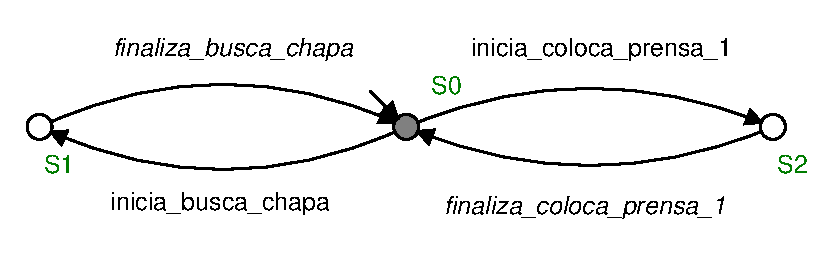
\includegraphics[width=\textwidth]{imagens/Robo_1.eps}
      \caption{Robô 1}
      \label{fig:robo1}
  \end{subfigure}
  \hfill
  \begin{subfigure}[b]{0.45\textwidth}
      \centering
      \includegraphics[width=\textwidth]{imagens/Robo_2.eps}
      \caption{Robô 2}
      \label{fig:robo2}
  \end{subfigure}
  \caption{Plantas robôs 1 e 2}
  \label{fig:robo12}
\end{figure}

O robô 3 possui as mesmas rotinas que o robô 2, porém ná prática assim que ele remove uma peça da prensa 2 ele precisa fazer o descarte dos retalhos, essa operação é feita internamente, assim que ele remove a peça da presa ele vai até à posição do descarte e libera as ventosas que seguram os retalhos, após isso vai para posição segura. 

O robô 4 possui uma rotina diferente, no sentido que ele não insere na prensa 4, ele leva a peça até o robô 5, pois na última operação a peça deve estar invertida, então para isso ser possível o robô 4 deve entregar a peça ao robô 5.
Logo o robô 4 possui as seguintes rotinas:

\begin{enumerate}
  \item Remove peça da prensa 3.
  \item Retorna para uma posição segura.
  \item Leva peça para o robô 5, onde ele só pode retornar assim que o robô 5 mandar sinal que já pegou a peça. 
  \item Retorno para um ponto seguro após entregar a peça.
  \item Em todos os estados é permitido a ocorrencia de evento de interrupção, o retorno da interrupção leva para um estado seguro inicial;
\end{enumerate}

A Figura \ref{fig:robo34} apresenta os modelos para os processos dos robôs 3 e 4.

\begin{figure}[H]%
  \centering
  \begin{subfigure}[b]{0.45\textwidth}
      \centering
      \includegraphics[width=\textwidth]{imagens/Robo_3.eps}
      \caption{Robô 3}
      \label{fig:robo3}
  \end{subfigure}
  \hfill
  \begin{subfigure}[b]{0.45\textwidth}
      \centering
      \includegraphics[width=\textwidth]{imagens/Robo_4.eps}
      \caption{Robô 4}
      \label{fig:robo4}
  \end{subfigure}
  \caption{Plantas robôs 3 e 4}
  \label{fig:robo34}
\end{figure}

Como descrito anteriormente o robô 5 pega a peça do robô 4, e ele faz a insereção e remoção na ultima prensa, podemos dividir as rotinas dele em:

\begin{enumerate}
  \item Pegar peça do robô 4, onde o mesmo vai chegar na posição onde o robô 4 vai largar a peça.
  \item Insere a peça na prensa, voltando a uma posição segura para que a prensa possa realizar o trabalho.
  \item Retirar a peça depois que a prensa finaliza o trabalho, nessa retirada da peça é feito também a lubrificação da prensa.
  \item Ao final a peça é levada até uma esteira onde é feito o descarte da mesma.
  \item Em todos os estados é permitido a ocorrencia de evento de interrupção, o retorno da interrupção leva para um estado seguro inicial;
\end{enumerate}

A Figura \ref{fig:robo5} apresenta o modelo para o processo do robô 5.

\begin{figure}[H]%
    \centering
    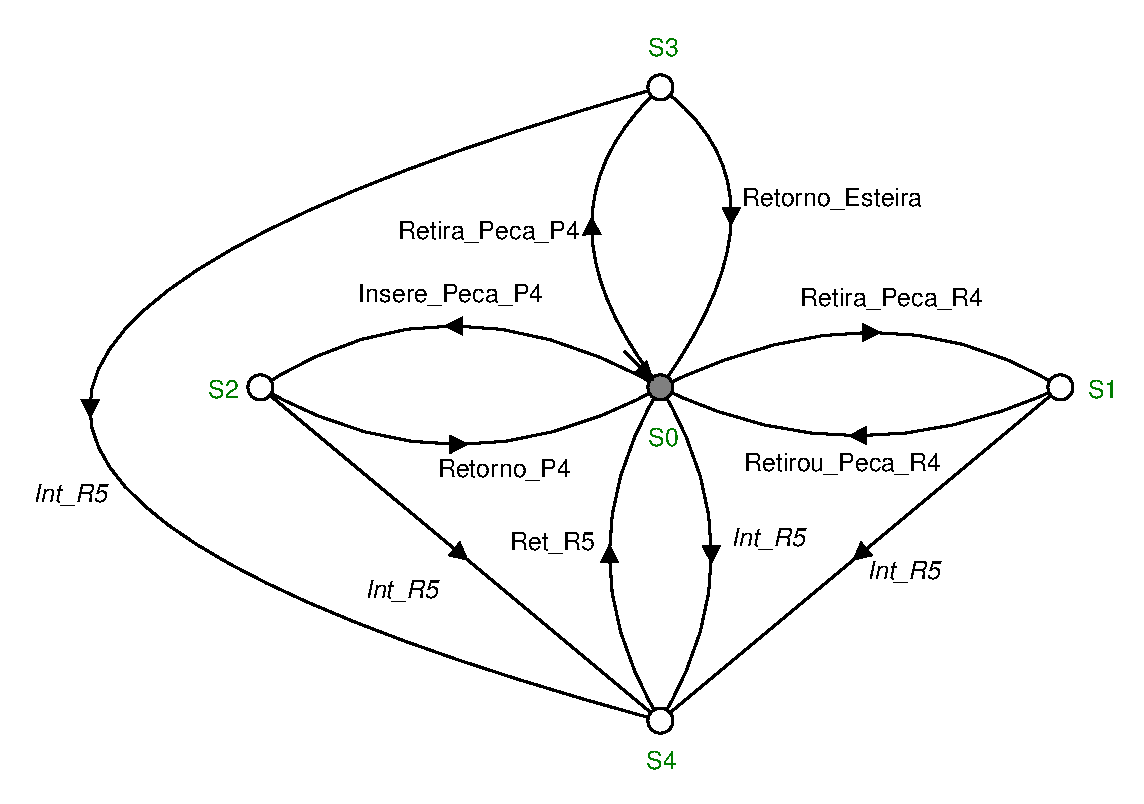
\includegraphics[width=0.9\textwidth]{imagens/robo_5.eps}
    \caption{Planta robô 5}\label{fig:robo5}
\end{figure}

As prensas funcionam da mesma maneira, tendo um acionador denotado por Bimanual, que quando acionado liga o motor fazendo com que ela movimente linearmente na vertical, subindo e descendo, a prensa possui alguns sinais internos para identificar o posicionamento sendo eles:

\begin{enumerate}
  \item PMS, ponto morto superior, este sinal é enviado quando o martelo da prensa esta na parte superior.
  \item PMI, ponto morto inferior, este sinal é enviado quando o martelo da prensa esta na parte inferior.
  \item Bimanual, sinal para acionar o motor da prensa para ela realizar o movimento.
  \item Após início de operação pode ocorrer evento de interrupção, o retorno da interrupção leva para um estado seguro inicial.
\end{enumerate}

É considerado um ciclo completo de trabalho quando a prensa passa do $PMS \to PMI \to PMS$. 

\begin{figure}[H]%
    \centering
    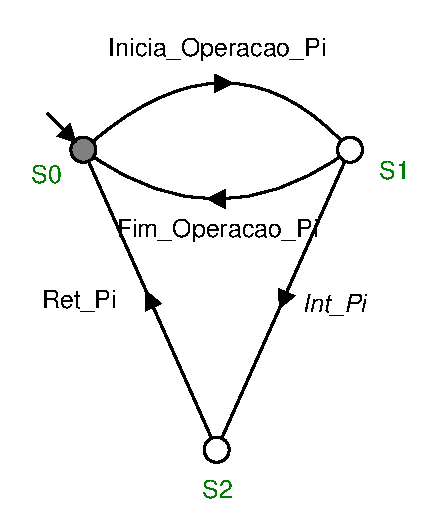
\includegraphics[width=0.6\textwidth]{imagens/Prensa.eps}
    \caption{Planta Prensa}\label{fig:prensa}
\end{figure}

\subsection{Especificações}
A seção a seguir apresenta as especificações desenvolvidas para cumprir com os requisitos de controle desejados.

A especificação apresentada na Figura \ref{fig:e0} permite ao robô 1 retirar peças da mesa centralizadora após o sensor detectar existencia de peça sobre a mesa.
Já a especificação apresentada na Figura \ref{fig:e1} limita o robô 1 a iniciar o processo de inserção na Prensa 1 após ter peça presente na garra.

\begin{figure}[H]%
  \centering
  \begin{subfigure}[b]{0.45\textwidth}
      \centering
      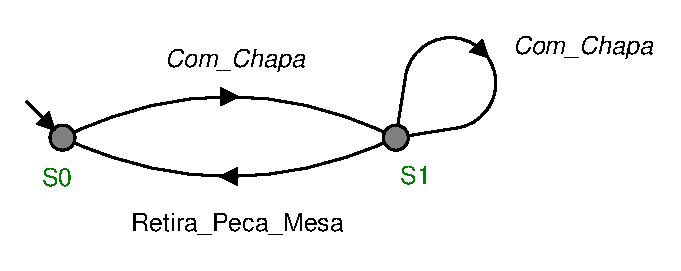
\includegraphics[width=\textwidth]{imagens/E0.eps}
      \caption{E0}
      \label{fig:e0}
  \end{subfigure}
  \hfill
  \begin{subfigure}[b]{0.45\textwidth}
      \centering
      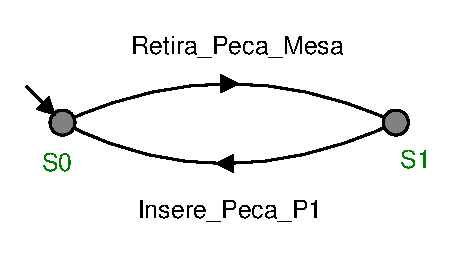
\includegraphics[width=\textwidth]{imagens/E1.eps}
      \caption{E1}
      \label{fig:e1}
  \end{subfigure}
  \caption{Especificações 0 e 1}
  \label{fig:e01}
\end{figure}

A especificação apresentada na Figura \ref{fig:e2} permite que a Prensa 1 inicie a operação após o robô 1 finalizar a inserção e estar em posição segura.
Já a especificação apresentada na \ref{fig:e3} é o modelo para overflow da Prensa 1 e libera uma nova inserção após a retirada da peça pelo robô 2.

\begin{figure}[H]%
  \centering
  \begin{subfigure}[b]{0.45\textwidth}
      \centering
      \includegraphics[width=\textwidth]{imagens/E2.eps}
      \caption{E2}
      \label{fig:e2}
  \end{subfigure}
  \hfill
  \begin{subfigure}[b]{0.45\textwidth}
      \centering
      \includegraphics[width=\textwidth]{imagens/E3.eps}
      \caption{E3}
      \label{fig:e3}
  \end{subfigure}
  \caption{Especificações 2 e 3}
  \label{fig:e23}
\end{figure}

A especificação apresentada na Figura \ref{fig:e4} limita o robô 2 a retirar peça da Prensa 1 após o final da operação.
Já a especificação apresentada na \ref{fig:e5} limita o robô 2 a iniciar o processo de inserção na Prensa 2 após ter peça presente na garra.

\begin{figure}[H]%
  \centering
  \begin{subfigure}[b]{0.45\textwidth}
      \centering
      \includegraphics[width=\textwidth]{imagens/E4.eps}
      \caption{E4}
      \label{fig:e4}
  \end{subfigure}
  \hfill
  \begin{subfigure}[b]{0.45\textwidth}
      \centering
      \includegraphics[width=\textwidth]{imagens/E5.eps}
      \caption{E5}
      \label{fig:e5}
  \end{subfigure}
  \caption{Especificações 4 e 5}
  \label{fig:e45}
\end{figure}

A especificação apresentada na Figura \ref{fig:e6} permite que a Prensa 2 inicie a operação após o robô 2 finalizar a inserção e estar em posição segura.
Já a especificação apresentada na \ref{fig:e7} é o modelo para overflow da Prensa 2 e libera uma nova inserção após a retirada da peça pelo robô 3.

\begin{figure}[H]%
  \centering
  \begin{subfigure}{0.45\textwidth}
      \centering
      \includegraphics[width=\textwidth]{imagens/E6.eps}
      \caption{E6}
      \label{fig:e6}
  \end{subfigure}
  \hfill
  \begin{subfigure}{0.45\textwidth}
      \centering
      \includegraphics[width=\textwidth]{imagens/E7.eps}
      \caption{E7}
      \label{fig:e7}
  \end{subfigure}
  \caption{Especificações 6 e 7}
  \label{fig:e67}
\end{figure}

A especificação apresentada na Figura \ref{fig:e8} limita o robô 3 a retirar peça da Prensa 2 após o final da operação.
Já a especificação apresentada na \ref{fig:e9} limita o robô 3 a iniciar o processo de inserção na Prensa 3 após ter peça presente na garra..

\begin{figure}[H]%
  \centering
  \begin{subfigure}{0.45\textwidth}
      \centering
      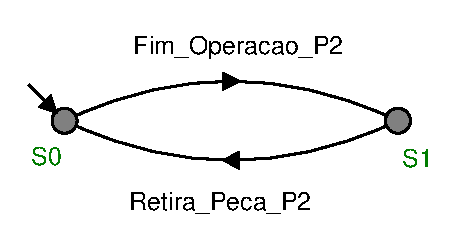
\includegraphics[width=\textwidth]{imagens/E8.eps}
      \caption{E8}
      \label{fig:e8}
  \end{subfigure}
  \hfill
  \begin{subfigure}{0.45\textwidth}
      \centering
      \includegraphics[width=\textwidth]{imagens/E9.eps}
      \caption{E9}
      \label{fig:e9}
  \end{subfigure}
  \caption{Especificações 8 e 9}
  \label{fig:e89}
\end{figure}

A especificação apresentada na Figura \ref{fig:e10} permite que a Prensa 3 inicie a operação após o robô 3 finalizar a inserção e estar em posição segura.
Já a especificação apresentada na \ref{fig:e11} é o modelo para overflow da Prensa 3 e libera uma nova inserção após a retirada da peça pelo robô 4.

\begin{figure}[H]%
  \centering
  \begin{subfigure}{0.45\textwidth}
      \centering
      \includegraphics[width=\textwidth]{imagens/E10.eps}
      \caption{E10}
      \label{fig:e10}
  \end{subfigure}
  \hfill
  \begin{subfigure}{0.45\textwidth}
      \centering
      \includegraphics[width=\textwidth]{imagens/E11.eps}
      \caption{E11}
      \label{fig:e11}
  \end{subfigure}
  \caption{Especificações 10 e 11}
  \label{fig:e1011}
\end{figure}

A especificação apresentada na Figura \ref{fig:e12} limita o robô 4 a retirar peça da Prensa 3 após o final da operação.
Já a especificação apresentada na \ref{fig:e13} limita o robô 4 a iniciar o processo de entrega para robô 5 após ter peça presente na garra.

\begin{figure}[H]%
  \centering
  \begin{subfigure}{0.45\textwidth}
      \centering
      \includegraphics[width=\textwidth]{imagens/E12.eps}
      \caption{E12}
      \label{fig:e12}
  \end{subfigure}
  \hfill
  \begin{subfigure}{0.45\textwidth}
      \centering
      \includegraphics[width=\textwidth]{imagens/E13.eps}
      \caption{E13}
      \label{fig:e13}
  \end{subfigure}
  \caption{Especificações 12 e 13}
  \label{fig:e1213}
\end{figure}

A especificação apresentada na Figura \ref{fig:e14} permite que a Prensa 4 inicie a operação após o robô 5 finalizar a inserção e estar em posição segura.
Já a especificação apresentada na \ref{fig:e15} limita o robô 5 a retirar peça da Prensa 5 após o final da operação.

\begin{figure}[H]%
  \centering
  \begin{subfigure}{0.45\textwidth}
      \centering
      \includegraphics[width=\textwidth]{imagens/E14.eps}
      \caption{E14}
      \label{fig:e14}
  \end{subfigure}
  \hfill
  \begin{subfigure}{0.45\textwidth}
      \centering
      \includegraphics[width=\textwidth]{imagens/E15.eps}
      \caption{E15}
      \label{fig:e15}
  \end{subfigure}
  \caption{Especificações 14 e 15}
  \label{fig:e1415}
\end{figure}

A especificação apresentada na Figura \ref{fig:e16} força robô 4 ao entregar uma peça aguarde o movimento do robô 5 de buscar a peça.
Já a especificação apresentada na \ref{fig:e17} força o robô 4 a aguardar posição segura do robô 5 para retornar do movimento de entrega de peça.

\begin{figure}[H]%
  \centering
  \begin{subfigure}{0.45\textwidth}
      \centering
      \includegraphics[width=\textwidth]{imagens/E16.eps}
      \caption{E16}
      \label{fig:e16}
  \end{subfigure}
  \hfill
  \begin{subfigure}{0.45\textwidth}
      \centering
      \includegraphics[width=\textwidth]{imagens/E17.eps}
      \caption{E17}
      \label{fig:e17}
  \end{subfigure}
  \caption{Especificações 16 e 17}
  \label{fig:e1617}
\end{figure}

A especificação apresentada na Figura \ref{fig:e18} limita o robô 5 a iniciar o processo de inserção na Prensa 4 após ter peça presente na garra.
Já a especificação apresentada na \ref{fig:e19} permite que o robô 5 pegue uma nova peça do robô 4 após entregar a peça manufaturada na esteira.

\begin{figure}[H]%
  \centering
  \begin{subfigure}{0.45\textwidth}
      \centering
      \includegraphics[width=\textwidth]{imagens/E18.eps}
      \caption{E18}
      \label{fig:e18}
  \end{subfigure}
  \hfill
  \begin{subfigure}{0.45\textwidth}
      \centering
      \includegraphics[width=\textwidth]{imagens/E19.eps}
      \caption{E19}
      \label{fig:e19}
  \end{subfigure}
  \caption{Especificações 18 e 19}
  \label{fig:e1819}
\end{figure}

\subsection{Solução modular de controle}
O software Supremica \cite{Supremica2020} disponibiliza funcionalidade para verificação da modularidade dos modelos desenvolvidos.
A Figura \ref{fig:modulare0} apresenta o resultado da análise da modularidade da especificação E0 com as plantas, podemos verificar que a especificação realiza controle de eventos sobre o robô 1 e sobre Sensor Chapa sem ter dependencia com outras plantas.

\begin{figure}[H]%
  \centering
  \includegraphics[width=0.8\textwidth]{imagens/modular_E0.eps}
  \caption{Estrutura modular para E0}\label{fig:modulare0}
\end{figure}

O processo de verificação de modularidade foi executado para todas as especificações, a tabela \ref{tab:modulos} apresenta o resultado para cada especificação e as respectivas plantas com atuação.
Foi verificado que o número máximo de interações de uma especificações é com duas plantas.

\begin{table}[h]%
\begin{center}
\begin{minipage}{0.5\textwidth}
\caption{Relações entre plantas e especificações}
\label{tab:modulos}
\begin{tabular}{@{}lll@{}}
  \toprule
  Especificação &  Planta 1 & Planta 2\\
  \midrule
  E0 & Sensor Chapa & Robô 1\\
  E1 & Robô 1 & \\
  E2 & Robô 1 & Prensa 1\\
  E3 & Robô 1 & Robô 2\\
  E4 & Robô 2 & Prensa 1\\
  E5 & Robô 2 & \\
  E6 & Robô 2 & Prensa 2\\
  E7 & Robô 2 & Robô 3\\
  E8 & Robô 3 & Prensa 2\\
  E9 & Robô 3 & \\
  E10 & Robô 3 & Prensa 3\\
  E11 & Robô 3 & Robô 4\\
  E12 & Robô 4 & Prensa 3\\
  E13 & Robô 4 & \\
  E14 & Robô 5 & Prensa 4\\
  E15 & Robô 5 & Prensa 4\\
  E16 & Robô 4 & Robo 5\\
  E17 & Robô 4 & Robo 5\\
  E18 & Robô 5 & \\
  E19 & Robô 5 & \\
  \botrule
\end{tabular}
\end{minipage}
\end{center}
\end{table}

Utilizando-se da relação entre especificações e plantas foi calculado o supervisor não bloqueante e controlavel modularmente para cada especificação.
A Tabela \ref{tab:supervisor} apresenta o número de estados, transições e eventos para cada supervisor modular e para o supervisor final.

\begin{table}[h]%
\begin{center}
\begin{minipage}{0.5\textwidth}
\caption{Supervisores Modulares}
\label{tab:supervisor}
\begin{tabular}{@{}llll@{}}
  \toprule
  Supervisor & Estados & Eventos & Transições\\
  \midrule
  Sup 0 & 8 & 7 & 23\\
  Sup 1 & 6 & 6 & 10\\
  Sup 2 & 24 & 10 & 73\\
  Sup 3 & 32 & 12 & 120\\
  Sup 4 & 24 & 10 & 73\\
  Sup 5 & 6 & 6 & 10\\
  Sup 6 & 24 & 10 & 73\\
  Sup 7 & 32 & 12 & 120\\
  Sup 8 & 24 & 10 & 73\\
  Sup 9 & 6 & 6 & 10\\
  Sup 10 & 24 & 10 & 73\\
  Sup 11 & 32 & 12 & 120\\
  Sup 12 & 24 & 10 & 73\\
  Sup 13 & 6 & 6 & 10\\
  Sup 14 & 30 & 12 & 98\\
  Sup 15 & 30 & 12 & 98\\
  Sup 16 & 40 & 14 & 159\\
  Sup 17 & 40 & 14 & 159\\
  Sup 18 & 9 & 8 & 18\\
  Sup 19 & 9 & 8 & 18\\
  %\midrule
  %\textbf{Final} & & &\\
  \botrule
\end{tabular}
\end{minipage}
\end{center}
\end{table}

Por limitação computacional não foi possivel realizar a composição de todos os supervisores para obtenção do controlador final, isso se deu devido à explosão do número de estados.
